\section{Evaluation protocol}
\label{sec:protocol}

\subsection{Folds, fits and cross-fitting}
All experiments use five stratified folds (seed 42) and, for confirmations, a second five-fold
split (seed 2026). Every learned transform --- medians for imputation, category vocabularies,
target encodings, word frequencies --- is fitted on the training part of the fold only. Target
statistics use \texttt{sklearn}'s \texttt{TargetEncoder} with \texttt{smooth='auto'} and an inner
five-fold cross-fit \citep{miccibarreca2001}, so a training row never sees its own label
through the encoding. Each fold yields out-of-fold probabilities; the headline number is the
mean of the five fold scores, and we also report the pooled out-of-fold \auc{}.

\subsection{Paired inference and the noise floor}
Two models scored on the same out-of-fold predictions are highly correlated, so the relevant
uncertainty is the standard error of their \emph{difference}. We use the DeLong placement-value
covariance \citep{delong1988}, which gives a closed form for
$\mathrm{SE}[\widehat{\mathrm{AUC}}_a-\widehat{\mathrm{AUC}}_b]$. On this data set the single-model
\auc{} has a standard error of about $8.5\times10^{-4}$, but the paired standard error of a
difference is only \dlt{2.2}--\dlt{2.7}. That number is the resolution of the whole study:
\emph{any change below $2.2\times10^{-4}$ cross-validated is indistinguishable from noise on one
five-fold split.} For comparison, retraining the same model with a different seed moves the
five-fold mean by \dlt{0.9} and the public score by \dlt{1.2}, which agrees.

\subsection{An adoption rule fixed before the experiment}
To avoid the usual drift of adopting whatever looks better, the rule is written into the code
before a candidate is trained: a candidate is adopted only if it improves the mean fold \auc{}
on both splits with at least four of five folds ahead, and the paired test on the primary split
returns $p<0.10$. The threshold is deliberately looser than the $p<0.05$ used for scientific
claims, because ensembling is a variance-reduction mechanism with a known sign; but it still
blocks the $10^{-5}$-scale changes. When the owner of the repository overrode the rule, the
override was recorded in the model-selection file together with the observed $p$, which keeps
the audit trail honest.

\section{The single-model ceiling}
\label{sec:single}

\subsection{Baselines}
Table~\ref{tab:baselines} reports the five baselines under the protocol above. The gradient
boosting models are close to each other (LightGBM \citep{lightgbm_docs} 0.9586,
XGBoost \citep{chen2016} 0.9585, CatBoost \citep{prokhorenkova2018} 0.9577 with its default 500
iterations), the linear model is far behind on numeric ratings (0.9216), and the constant
predictor defines the trivial floor.

\begin{table}[t]
\centering
\small
\caption{Baselines on the five fixed folds. Mean and population standard deviation of the fold
\auc{}, pooled out-of-fold \auc{} and log loss.}
\label{tab:baselines}
\begin{tabular}{lcccc}
\toprule
Model & mean fold \auc{} & std & OOF \auc{} & OOF log loss\\
\midrule
Constant prior            & 0.50000 & 0.00000 & 0.50000 & 0.68677\\
Logistic regression       & 0.92156 & 0.00043 & 0.92156 & 0.34424\\
CatBoost (500 it.)        & 0.95770 & 0.00066 & 0.95770 & 0.23057\\
XGBoost (500 it.)         & 0.95846 & 0.00061 & 0.95845 & 0.22842\\
LightGBM (500 it.)        & 0.95862 & 0.00059 & 0.95861 & 0.22789\\
\bottomrule
\end{tabular}
\end{table}

\subsection{What moved the single model, and what did not}
The ladder in Figure~\ref{fig:progress}a starts at 0.9586 for a raw LightGBM. Adding five
crossed categorical features (travel$\times$cabin, cabin$\times$boarding, \ldots) gives
\dlt{1.6} and 16 Optuna trials \dlt{2.4}; both are inside or at the edge of the noise band. The
first large step is the cross-fitted target statistics of the flight-distance keys:
$+13.5$ \dlt{} ($p=5\times10^{-4}$), which is the only single change in the whole study that
clears the noise floor by a wide margin. Smoothing those encodings with the empirical-Bayes
default adds \dlt{1.65} ($p=0.46$); we kept it because it also minimised the tuned objective,
but we do not claim it is a real improvement.

Capacity is saturated. Doubling the number of trees (500 $\to$ 1{,}000) costs \dlt{0.9};
reducing the leaves from 63 to 31 costs \dlt{2.1}; a 127-leaf model at learning rate 0.03
peaks at 500 trees and then degrades; a 255-leaf model at rate 0.02 degrades monotonically
(0.9597 at 500 trees down to 0.9585 at 3{,}000). The validation curve flattens at about 400
trees. The sixteen Optuna trials that produced the adopted configuration are spread over
$9.5\times10^{-4}$, and the top two trials differ by $10^{-5}$ --- a ranking of noise.

\begin{figure}[t]
\centering
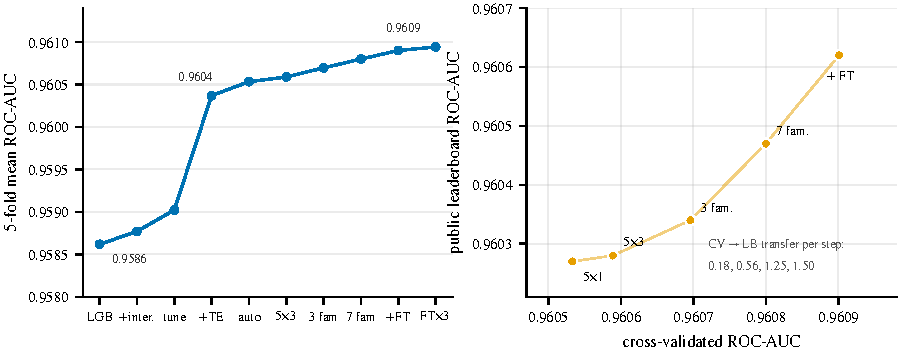
\includegraphics[width=\linewidth]{figures/fig_progress.pdf}
\caption{Left: five-fold mean \auc{} along the modelling path. Right: the same models on the
public leaderboard. Each submitted model sits about \dlt{3} below its cross-validated score ---
the constant offset between the two readings --- but the \emph{per-step} transfer grows with
the diversity of the ensemble.}
\label{fig:progress}
\end{figure}
